% -*- TeX -*- -*- UK -*- -*- Soft -*-

\part{Study Notes: Nelis Willers}

\chapter{Biological Systems}



\section{Biological Nervous Systems (BNSs)}

Branislav Holl\"{a}nder \cite{Hollander2018} wrote the text in this section.

Biological nervous systems, such as those found in vertebrates, operate in a different way. Take a look at the diagram. It shows a neuron cell connecting to another neuron. The cell consists of a cell body, with dendrites acting as connecting wires for other neurons to connect to. In most cases, a neuron has one axon capable of transmitting electric currents actively to other connecting cells. The connections between neurons are established using synapses located at the end of the axon. 
\begin{marginfigure}
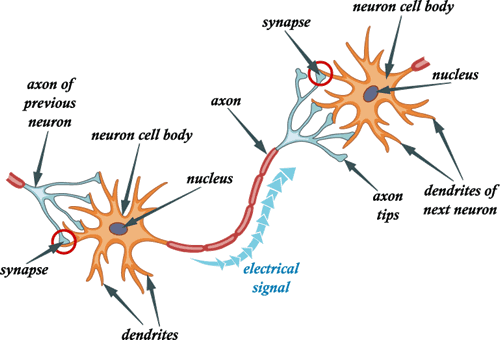
\includegraphics{biologicalneurons}
\end{marginfigure}

These synapses are responsible for a lot of the magic of computing and memory in the nervous system. To see how this works, let us first examine the response of a single neuron to an incoming signal from its dendrites\cite{Synaptidude2005}.
\begin{marginfigure}
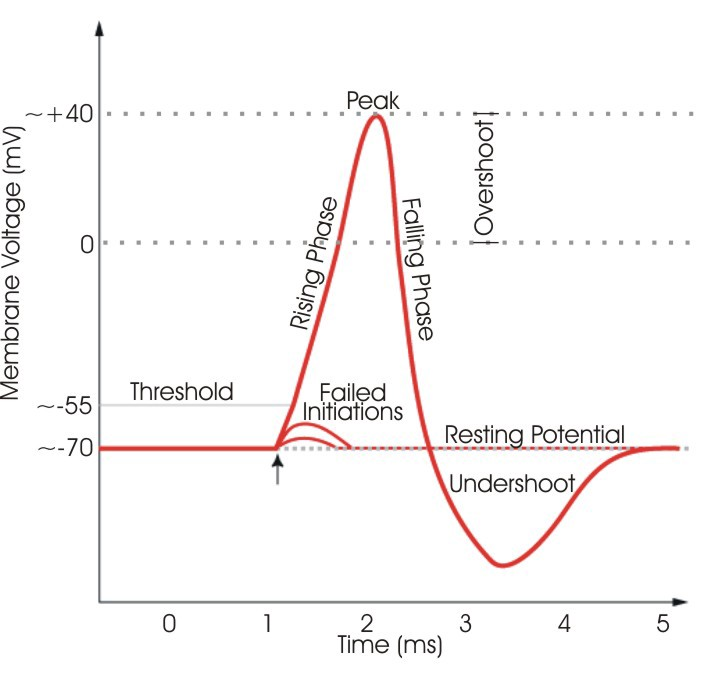
\includegraphics{biologicalneurons02}
\end{marginfigure}
We can observe that the synaptic membrane of the neuron typically has a resting potential of $-$70mV. In the resting state the cell does not carry any signal. In order to transmit a signal the cell has to be stimulated by its input synapses. In our example, the voltage threshold required to elicit a response is $-$55mV. This means that the total sum of the input has to amount to $+$15mV. If each input neuron only contributes $+$5mV, we need at least 3 such inputs to be active at the same time to provoke a response in the neuron. The mechanism is very similar to that of the artificial neurons in that the inputs get summed up before passing through a non-linearity. Inputs that cause a positive change in the membrane potential are called excitatory. In contrast to ANNs, in BNSs we can also find inhibitory inputs causing a negative change in the potential. These act to prevent the firing of an action potential.

We see that if the input is weaker than $+$15mV, there is no signal at the output. However, above the threshold, a strong active signal in generated, called the action potential. The potential rises sharply and is carried through the axon to the output synapses. After a short amount of time, the potential declines again. For some time after the decline, the cell may not be stimulated again (absolute refractory period).

The sharp thresholding of the input is equivalent to the non-linearity present in ANNs (the threshold in BNSs corresponds to a Heaviside non-linearity, just like in the early perceptron). Note that the firing of the action potential is binary: either it occurs or it does not. There is nothing in-between. This is called the all-or-nothing principle. Therefore, BNSs carry binary signals. This is in contrast to ANNs which carry continuous signals. However, the binary signals in NNNs are changing over time, which makes up for the reduced expressive power of binary values.

Of course, in order to transfer information in its binary form, BNSs have to use some kind of binary encoding, just as computers do. The most popular theories are that BNSs use frequency-based encoding and/or temporal encoding. In frequency-based encoding, the average frequency of impulses encodes the strength of a signal. Therefore, we might say that BNSs use frequency modulation. Notice that the average frequency is important in this mechanism, not the arrival time of individual impulses. This form of signal transfer is not very effective because it ignores the small time differences between individual impulses that could in principle carry information. However, frequency encoding is very robust to noise. Noise is a big concern in a electrochemical systems such as the nervous system.

Temporal encoding is similar to frequency encoding, except that the arrival time of individual impulses does matter in this case. A number of studies (see e.g. this paper) suggest that temporal encoding may be used at various places in our nervous system, such as in sensory systems. Temporal coding is very sensitive to noise, but may be necessary if a large amount of information needs to be transferred quickly.

The learning process of the human brain is not yet completely understood. However, we can say almost with certainty that the brain doesn't use a global learning method such as gradient descent. Gradient descent as is used in ANNs requires backpropagation. There is no biological mechanism for errors to be backpropagated further than a single neuron. Another issue is the definition of the loss function: do we as humans have inherent loss functions for various tasks defined in our brains? This is not very likely.

On the other hand, we found strong evidence (thanks largely to Eric Kandel, a Nobel laureate) that the brain is learning by using local methods such as Hebbian learning or \ac{STDP}. These methods are similar to learning in Restricted Boltzmann Machines in that they strengthen connections between neurons that often transmit signals between each other. The foundational concept of Hebbian learning is best explained by the author himself:

\begin{quote}
    Let us assume that the persistence or repetition of a reverberatory activity (or ``trace'') tends to induce lasting cellular changes that add to its stability. […] When an axon of cell A is near enough to excite a cell B and repeatedly or persistently takes part in firing it, some growth process or metabolic change takes place in one or both cells such that A's efficiency, as one of the cells firing B, is increased. (Hebb, D.O. (1949). The Organization of Behavior. New York: Wiley \& Sons.)
\end{quote}

STDP further enhances the Hebbian learning concept by making it time-asymmetric. More specifically, STDP strengthens the connection between neurons if input spikes in the first neuron occur immediately before output spikes in the second neuron. Otherwise, if the input spike of the first neuron occurs immediately after the output spike of the second neuron, the connection is weakened.

Hebbian learning is probably the most important learning mechanism occurring in the human brain. However, there is evidence that long-term memory may also work by regulating the presence/absence of connections between individual neurons, thus changing the very structure of the network. 

Despite of the current success of ANNs in the field of AI and Machine Learning, BNSs still exhibit multiple advantages, the most important being their extremely low power consumption. Current consensus among researchers suggests that the brain consumes approx. 20~W of energy. Compare that to an infinitely less capable Nvidia GPU consuming 300~W running a deep neural network. The low power consumption in turn requires much less cooling and allows the brain to build 3-D structures as opposed to electronic chips mostly following of 2-D designs.

Multiple research groups are currently trying to emulate some aspects of the nervous system \textit{in silico}. Such systems are called neuromorphic. Advantages of such systems should include, among others, high power efficiency, inherent massive parallelism and potentially real-time performance in inference. 